%%%%%%%% ICML 2019 EXAMPLE LATEX SUBMISSION FILE %%%%%%%%%%%%%%%%%

\documentclass{article}

% Recommended, but optional, packages for figures and better typesetting:
\usepackage{microtype}
\usepackage{graphicx}
\usepackage{subfigure}
\usepackage{booktabs} % for professional tables

% hyperref makes hyperlinks in the resulting PDF.
% If your build breaks (sometimes temporarily if a hyperlink spans a page)
% please comment out the following usepackage line and replace
% \usepackage{icml2019} with \usepackage[nohyperref]{icml2019} above.
\usepackage{hyperref}

% Attempt to make hyperref and algorithmic work together better:
\newcommand{\theHalgorithm}{\arabic{algorithm}}

% Use the following line for the initial blind version submitted for review:
\usepackage{icml2019}

% If accepted, instead use the following line for the camera-ready submission:
%\usepackage[accepted]{icml2019}

% The \icmltitle you define below is probably too long as a header.
% Therefore, a short form for the running title is supplied here:
\icmltitlerunning{Provable Overparameterized Neural Network Policy Gradient Method}

\usepackage{amssymb} %maths
\usepackage{amsmath} %maths
\usepackage{amsthm}
\usepackage{hyperref}
\usepackage[utf8]{inputenc} %useful to type directly diacritic characters
\usepackage[capitalize]{cleveref}
\crefname{prop}{Proposition}{Propositions}
\crefname{thm}{Theorem}{Theorems}
\crefname{lem}{Lemma}{Lemmas}


\def\rva{{\mathbf{a}}}
\def\rvo{{\mathbf{o}}}
\def\rvr{{\mathbf{r}}}
\def\rvs{{\mathbf{s}}}
\def\rvu{{\mathbf{u}}}
\def\rvw{{\mathbf{w}}}
\def\rvx{{\mathbf{x}}}
\def\rvg{{\mathbf{g}}}
\def\rvo{{\mathbf{o}}}
\def\rvone{{\mathbf{1}}}
\def\rvzero{{\mathbf{0}}}
\def\rvtilder{{\tilde{\mathbf{r}}}}

\def\rvp{{\mathbf{p}}}

\def\pr{{\text{Pr}}}
\def\r{{\text{R}}}

\def\regret{{\text{Regret}}}

\newtheorem{thm}{Theorem}
\newtheorem{lem}{Lemma}
\newtheorem{defi}{Definition}
\newtheorem{prop}{Proposition}
\newtheorem{remk}{Remark}


\def\rvpi{{\boldsymbol{\pi}}}

\def\rmI{{\mathbf{I}}}
\def\rmW{{\mathbf{W}}}
\def\rmX{{\mathbf{X}}}

\def\sE{{\mathbb{E}}}
\def\sR{{\mathbb{R}}}
\def\sI{{\mathbb{I}}}

\def\gN{{\mathcal{N}}}
\def\gE{{\mathcal{E}}}
\def\gU{{\mathcal{U}}}




\begin{document}

\twocolumn[
\icmltitle{Provable Overparameterized Neural Network Policy Gradient Method
}

% It is OKAY to include author information, even for blind
% submissions: the style file will automatically remove it for you
% unless you've provided the [accepted] option to the icml2019
% package.

% List of affiliations: The first argument should be a (short)
% identifier you will use later to specify author affiliations
% Academic affiliations should list Department, University, City, Region, Country
% Industry affiliations should list Company, City, Region, Country

% You can specify symbols, otherwise they are numbered in order.
% Ideally, you should not use this facility. Affiliations will be numbered
% in order of appearance and this is the preferred way.
\icmlsetsymbol{equal}{*}

\begin{icmlauthorlist}
\icmlauthor{Aeiau Zzzz}{equal,to}
\icmlauthor{Bauiu C.~Yyyy}{equal,to,goo}
\icmlauthor{Cieua Vvvvv}{goo}
\icmlauthor{Iaesut Saoeu}{ed}
\icmlauthor{Fiuea Rrrr}{to}
\icmlauthor{Tateu H.~Yasehe}{ed,to,goo}
\icmlauthor{Aaoeu Iasoh}{goo}
\icmlauthor{Buiui Eueu}{ed}
\icmlauthor{Aeuia Zzzz}{ed}
\icmlauthor{Bieea C.~Yyyy}{to,goo}
\icmlauthor{Teoau Xxxx}{ed}
\icmlauthor{Eee Pppp}{ed}
\end{icmlauthorlist}

\icmlaffiliation{to}{Department of Computation, University of Torontoland, Torontoland, Canada}
\icmlaffiliation{goo}{Googol ShallowMind, New London, Michigan, USA}
\icmlaffiliation{ed}{School of Computation, University of Edenborrow, Edenborrow, United Kingdom}

\icmlcorrespondingauthor{Cieua Vvvvv}{c.vvvvv@googol.com}
\icmlcorrespondingauthor{Eee Pppp}{ep@eden.co.uk}

% You may provide any keywords that you
% find helpful for describing your paper; these are used to populate
% the "keywords" metadata in the PDF but will not be shown in the document
\icmlkeywords{Machine Learning, ICML}

\vskip 0.3in
]

% this must go after the closing bracket ] following \twocolumn[ ...

% This command actually creates the footnote in the first column
% listing the affiliations and the copyright notice.
% The command takes one argument, which is text to display at the start of the footnote.
% The \icmlEqualContribution command is standard text for equal contribution.
% Remove it (just {}) if you do not need this facility.

%\printAffiliationsAndNotice{}  % leave blank if no need to mention equal contribution
\printAffiliationsAndNotice{\icmlEqualContribution} % otherwise use the standard text.

\begin{abstract}
In this paper, we provide theoretical analysis for policy gradient method, where the policy is parameterized by neural networks. We first show that in bandit setting, with two layered overparameterized ReLU neural net policy and enough exploration, policy gradient method achieves sublinear regret. For episodic Markov decision process setting, we then prove that similar results hold. The results can be generalized to policy parameterized by multil-layered neural networks.
\end{abstract}

\section{Introduction}
\label{submission}

Deep Reinforcement Learning (DRL) has recently achieved great successes in many fields, e.g, defeating professional players in Go, two player Hold'em, and Atari games, to name a few. However, comparing with its practical performance, the theoretical understanding and explanation of the mechanism behind its success is not enough.

Since DRL combines techniques of Deep Learning (DL) and Reinforcement Learning (RL), to understand DRL, we need to combine findings from both DL and RL sides.

On the RL side, it is well studied that under bandit setting and tabular cases of Markov decision process (MDP) setting, many popular algorithms enjoy favorable theoretical guarantees. In particular, either the algorithm converges asymptotically, or its regret of has finite time sublinear upper bound. However, once it goes beyond the tabular cases, the theoretical guarantee becomes weaker. For example, in linear function approximation, only fixed point property is known for the algorithm. Even worse, when we combine RL methods with non-linear neural networks, such as DQN algorithm, little is known in theory.

On the DL side, empirical achievements are also much more advanced than theoretical results. However, there are still progresses in the expressiveness, optimization, and generalization aspects of DL theory. In particular, very recently, it has been discovered that, in supervised learning (regression and classification) settings, the training loss can be globally optimized (in linear convergence rate for $\ell_2$ loss in regression, and in constant time for classification) by gradient descent (GD) and stochastic gradient descent (SGD) method, given that the number of parameters in hidden layer is quite large, i.e., overparameterization. With some additional structured data distribution assumptions, the convergent training loss can be generalized to testing loss, making the neural network have provable generalization ability. 

In this paper, based on the recent progresses in overparameterized neural network optimization, we make one step forward to theoretically understanding DRL. In particular, we make the following contributions.
\begin{itemize}
    \item We prove that in bandit setting, with enough exploration, the widely-used policy gradient method, with policy net represented by a overparameterized two layer neural network (NN), achieves $\tilde{O}\left( \sqrt{T} \right)$ regret.
    \item We show that in episodic MDP setting, with the same exploration strategy and policy net as above, policy gradient method achieves $\tilde{O}\left( \sqrt{T} \right)$ regret.
    \item In many state dependent bandit and MDP settings, similar results also hold.
\end{itemize}

We would like to point that the above results can be generalized to policy net represented by multi-layered neural networks. Assuming a two layer NN policy is just for simplicity and conciseness. We provide the generalization to multi-layered NN for completeness.

To our knowledge, our finding is the first convergence result for popular RL methods (here, policy gradient) with non-linear NN function approximations, which provides theoretical support for DRL methods. Our result is just beginning of understanding many other DRL methods (like DQN, A3C, PCL, etc), with more practical NN function approximations (e.g., less overparameterized), using many other policy optimization techniques (such as mirror descent, and relative entropy policy search).

The rest of the paper is organized as follows. Some proofs are deferred to appendix due to space limit.

\subsection{Notations}

Bold letters refer to vectors, and non-bold letters refer to scalars. For example, $u_{i,r} \in \sR$ is the $r$th component of vector $\rvu_i \in \sR^m$. $n$ is the total number of data points, while $m$ is the total number of nodes in each hidden layer. $h$ is the total number of arms/trajectories of each bandit/starting state.

\begin{itemize}
	\item $\rvs_i \in \sR^d$, $i \in [n]$ is a state/bandit.
	\item $\rvw_r \in \sR^d$, $r \in [m]$ is a weight vector in the first hidden layer.
	\item $u_{i,r} \triangleq \sigma(\rvw_r^\top \rvs_i)$, where $\sigma(\cdot) \triangleq \max\left\{ \cdot, 0 \right\}$ is the ReLU activation function.
	\item $\rva_k \in \sR^m$, $k \in [h]$ is a weight vector in the second layer. $\rva_k \sim \gN(0, \rmI)$.
	\item $o_{i,k} \triangleq \sum\limits_{r=1}^{m}{a_{k,r} \cdot u_{i,r}}$ is the logit of the $k$th arm for state $\rvs_i$.
	\item $\pi_{i,k} \triangleq \frac{\exp\left\{ o_{i,k} \right\}}{\sum\limits_{k^\prime = 1}^{h}{\exp\left\{ o_{i,k^\prime} \right\}}}$ is the  probability for choosing arm $k$ in bandit $i$.
	\item $\rvr_i \in \sR^h$ is the reward vector for bandit $i$.
	\item $\r_i^{\max} \triangleq \max\limits_{k}\left\{ r_{i,k} \right\}$ is the maximum reward of bandit $i$.
	\item The loss/regret $\ell \triangleq \regret(\rvpi) \triangleq \frac{1}{n} \cdot \sum\limits_{i=1}^{n}{ \left( \r_i^{\max} - \rvpi_i^\top \rvr_i \right) }$. Regret minimization is equivalent with maximizing reward $\frac{1}{n} \sum\limits_{i=1}^{n}{\rvpi_i^\top \rvr_i}$.
\end{itemize}

Denote $\rvtilder_{i} \triangleq \r_i^{\max} \cdot \rvone -  \rvr_{i} \ge \rvzero$. The regret at time step $t$ is,
\begin{equation*}
\begin{split}
	\ell(t) \triangleq \regret(\rvpi(t)) &= \frac{1}{n} \cdot \sum\limits_{i=1}^{n}{ \left( \r_i^{\max} - \rvpi_{i}(t)^\top \rvr_i \right) } \\
	&= \frac{1}{n} \cdot \sum\limits_{i=1}^{n}{ \rvpi_{i}(t)^\top \left( \r_i^{\max} \cdot \rvone - \rvr_{i} \right) } \\
	&= \frac{1}{n} \cdot \sum\limits_{i=1}^{n}{ \rvpi_{i}(t)^\top \rvtilder_{i} }.
\end{split}
\end{equation*}

\section{Main Results}

\subsection{Settings}

\subsubsection{Bandit}

We first analyze the standard bandit setting, i.e., $n = 1$ , and then generalize the results to many state dependent bandits setting. For simplicity, assume the reward $\rvr \in \sR^h$ is a deterministic vector. Using concentration the results can be generalized to random reward vectors, therefore recovering the stochastic bandit setting. Also we assume $r_k \in [0, 1]$, $\forall k \in [h]$.

In this setting, we use the NN policy to pull one arm $A_t \in [h]$ in each time step $t$, then observe the reward $r_{A_t}$. The policy net then uses the reward to update its weight vectors, using policy gradient method. After such $T$ steps, we are concerned with the regret,
\begin{equation*}
    \ell \triangleq \regret(\rvpi) \triangleq \r^{\max} \cdot T - \sum\limits_{t=0}^{T-1}{ \rvpi(t)^\top \rvr } = \sum\limits_{t=0}^{T-1}{ \rvpi(t)^\top \rvtilder }
\end{equation*}

\subsubsection{Episodic MDP}

In the Episodic MDP setting, in each time step, we use NN policy to take one action $A_t$, then observe a reward $R_{t+1}$ and next state $S_{t+1}$. After such $H$ steps, there is an ending state, and this trajectory terminates. Since we use policy gradient method (no value learning method here), the policy updates its weights using the cumulative reward collected from each trajectory. 


\subsection{Policy Gradient Method}

\begin{algorithm}[h]
   \caption{Policy Gradient Method Mixed with Uniform Exploration}
   \label{alg:example}
\begin{algorithmic}
   \STATE {\bfseries Input:} state feature vectors $\rvs_i$
   \STATE Initialize $\rvw_r \sim \gN\left( 0, \sigma \cdot \rmI \right)$, $\forall r \in [m]$, $\rva_k \sim \gN(0, \rmI)$, $\forall k \in [h]$.
   \FOR{$t=0$ {\bfseries to} $T-1$}
   \IF{$t < \sqrt{T}$}
   \STATE Uniformly randomly take action $A_{i,t}$. 
   \STATE Observe reward and next state.
   \ELSE
   \STATE Take action $A_{i,t} \sim \rvpi_{i}\left(\cdot \middle| S_{i,t} \right)$. 
   \ENDIF
   \STATE $\rvw_r(t+1) = \rvw_r(t) - \eta \cdot \frac{d\ell}{d \rvw_r(t)}$, $\forall r \in [m]$.
   \ENDFOR
\end{algorithmic}
\end{algorithm}

The objective of our analysis is the policy gradient method, mixed with uniform exploration. The reason why we need exploration will be explained later on, and technically it seems cannot be eliminated.

You can use footnotes\footnote{Footnotes
should be complete sentences.} to provide readers with additional
information about a topic without interrupting the flow of the paper.
Indicate footnotes with a number in the text where the point is most
relevant. Place the footnote in 9~point type at the bottom of the
column in which it appears. Precede the first footnote in a column
with a horizontal rule of 0.8~inches.\footnote{Multiple footnotes can
appear in each column, in the same order as they appear in the text,
but spread them across columns and pages if possible.}

\begin{figure}[ht]
\vskip 0.2in
\begin{center}
\centerline{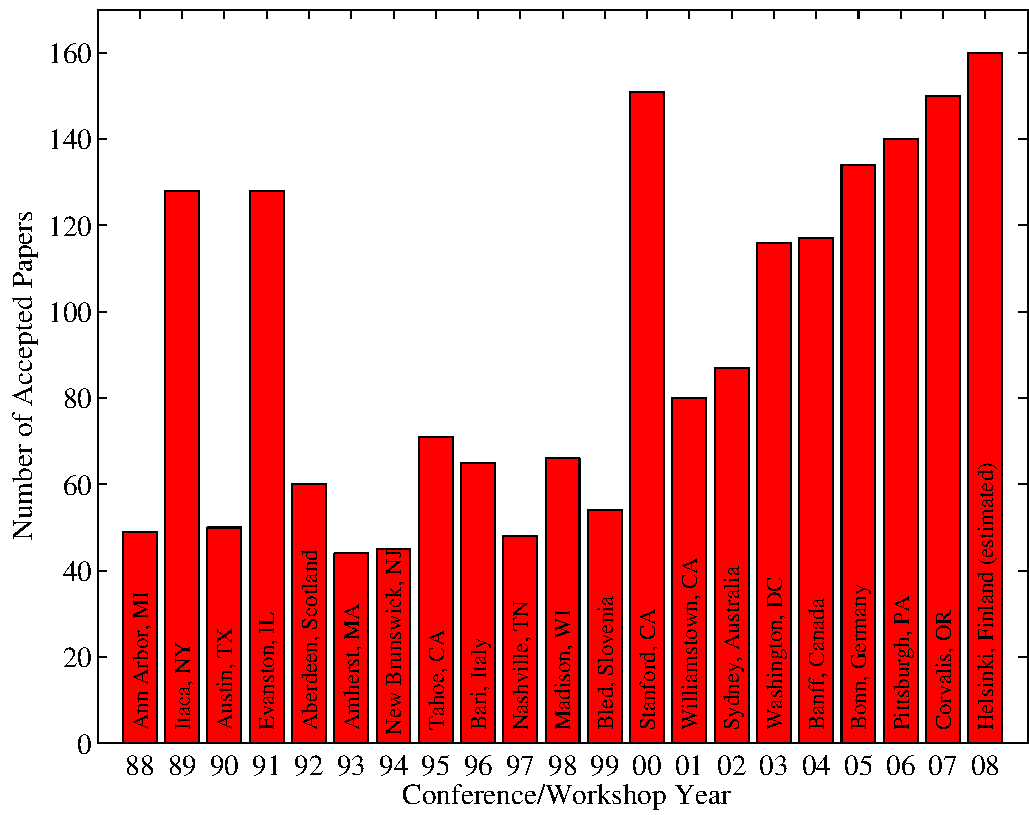
\includegraphics[width=\columnwidth]{icml_numpapers}}
\caption{Historical locations and number of accepted papers for International
Machine Learning Conferences (ICML 1993 -- ICML 2008) and International
Workshops on Machine Learning (ML 1988 -- ML 1992). At the time this figure was
produced, the number of accepted papers for ICML 2008 was unknown and instead
estimated.}
\label{icml-historical}
\end{center}
\vskip -0.2in
\end{figure}

\subsection{Figures}

You may want to include figures in the paper to illustrate
your approach and results. Such artwork should be centered,
legible, and separated from the text. Lines should be dark and at
least 0.5~points thick for purposes of reproduction, and text should
not appear on a gray background.

Label all distinct components of each figure. If the figure takes the
form of a graph, then give a name for each axis and include a legend
that briefly describes each curve. Do not include a title inside the
figure; instead, the caption should serve this function.

Number figures sequentially, placing the figure number and caption
\emph{after} the graphics, with at least 0.1~inches of space before
the caption and 0.1~inches after it, as in
Figure~\ref{icml-historical}. The figure caption should be set in
9~point type and centered unless it runs two or more lines, in which
case it should be flush left. You may float figures to the top or
bottom of a column, and you may set wide figures across both columns
(use the environment \texttt{figure*} in \LaTeX). Always place
two-column figures at the top or bottom of the page.

\subsection{Algorithms}

If you are using \LaTeX, please use the ``algorithm'' and ``algorithmic''
environments to format pseudocode. These require
the corresponding stylefiles, algorithm.sty and
algorithmic.sty, which are supplied with this package.
Algorithm~\ref{alg:example} shows an example.

\begin{algorithm}[tb]
   \caption{Bubble Sort}
   \label{alg:example}
\begin{algorithmic}
   \STATE {\bfseries Input:} data $x_i$, size $m$
   \REPEAT
   \STATE Initialize $noChange = true$.
   \FOR{$i=1$ {\bfseries to} $m-1$}
   \IF{$x_i > x_{i+1}$}
   \STATE Swap $x_i$ and $x_{i+1}$
   \STATE $noChange = false$
   \ENDIF
   \ENDFOR
   \UNTIL{$noChange$ is $true$}
\end{algorithmic}
\end{algorithm}

\subsection{Tables}

You may also want to include tables that summarize material. Like
figures, these should be centered, legible, and numbered consecutively.
However, place the title \emph{above} the table with at least
0.1~inches of space before the title and the same after it, as in
Table~\ref{sample-table}. The table title should be set in 9~point
type and centered unless it runs two or more lines, in which case it
should be flush left.

% Note use of \abovespace and \belowspace to get reasonable spacing
% above and below tabular lines.

\begin{table}[t]
\caption{Classification accuracies for naive Bayes and flexible
Bayes on various data sets.}
\label{sample-table}
\vskip 0.15in
\begin{center}
\begin{small}
\begin{sc}
\begin{tabular}{lcccr}
\toprule
Data set & Naive & Flexible & Better? \\
\midrule
Breast    & 95.9$\pm$ 0.2& 96.7$\pm$ 0.2& $\surd$ \\
Cleveland & 83.3$\pm$ 0.6& 80.0$\pm$ 0.6& $\times$\\
Glass2    & 61.9$\pm$ 1.4& 83.8$\pm$ 0.7& $\surd$ \\
Credit    & 74.8$\pm$ 0.5& 78.3$\pm$ 0.6&         \\
Horse     & 73.3$\pm$ 0.9& 69.7$\pm$ 1.0& $\times$\\
Meta      & 67.1$\pm$ 0.6& 76.5$\pm$ 0.5& $\surd$ \\
Pima      & 75.1$\pm$ 0.6& 73.9$\pm$ 0.5&         \\
Vehicle   & 44.9$\pm$ 0.6& 61.5$\pm$ 0.4& $\surd$ \\
\bottomrule
\end{tabular}
\end{sc}
\end{small}
\end{center}
\vskip -0.1in
\end{table}

Tables contain textual material, whereas figures contain graphical material.
Specify the contents of each row and column in the table's topmost
row. Again, you may float tables to a column's top or bottom, and set
wide tables across both columns. Place two-column tables at the
top or bottom of the page.

\subsection{Citations and References}

Please use APA reference format regardless of your formatter
or word processor. If you rely on the \LaTeX\/ bibliographic
facility, use \texttt{natbib.sty} and \texttt{icml2019.bst}
included in the style-file package to obtain this format.

Citations within the text should include the authors' last names and
year. If the authors' names are included in the sentence, place only
the year in parentheses, for example when referencing Arthur Samuel's
pioneering work \yrcite{Samuel59}. Otherwise place the entire
reference in parentheses with the authors and year separated by a
comma \cite{Samuel59}. List multiple references separated by
semicolons \cite{kearns89,Samuel59,mitchell80}. Use the `et~al.'
construct only for citations with three or more authors or after
listing all authors to a publication in an earlier reference \cite{MachineLearningI}.

Authors should cite their own work in the third person
in the initial version of their paper submitted for blind review.
Please refer to Section~\ref{author info} for detailed instructions on how to
cite your own papers.

Use an unnumbered first-level section heading for the references, and use a
hanging indent style, with the first line of the reference flush against the
left margin and subsequent lines indented by 10 points. The references at the
end of this document give examples for journal articles \cite{Samuel59},
conference publications \cite{langley00}, book chapters \cite{Newell81}, books
\cite{DudaHart2nd}, edited volumes \cite{MachineLearningI}, technical reports
\cite{mitchell80}, and dissertations \cite{kearns89}.

Alphabetize references by the surnames of the first authors, with
single author entries preceding multiple author entries. Order
references for the same authors by year of publication, with the
earliest first. Make sure that each reference includes all relevant
information (e.g., page numbers).

Please put some effort into making references complete, presentable, and
consistent. If using bibtex, please protect capital letters of names and
abbreviations in titles, for example, use \{B\}ayesian or \{L\}ipschitz
in your .bib file.

\subsection{Software and Data}

We strongly encourage the publication of software and data with the
camera-ready version of the paper whenever appropriate. This can be
done by including a URL in the camera-ready copy. However, do not
include URLs that reveal your institution or identity in your
submission for review. Instead, provide an anonymous URL or upload
the material as ``Supplementary Material'' into the CMT reviewing
system. Note that reviewers are not required to look at this material
when writing their review.

% Acknowledgements should only appear in the accepted version.
\section*{Acknowledgements}

\textbf{Do not} include acknowledgements in the initial version of
the paper submitted for blind review.

If a paper is accepted, the final camera-ready version can (and
probably should) include acknowledgements. In this case, please
place such acknowledgements in an unnumbered section at the
end of the paper. Typically, this will include thanks to reviewers
who gave useful comments, to colleagues who contributed to the ideas,
and to funding agencies and corporate sponsors that provided financial
support.


% In the unusual situation where you want a paper to appear in the
% references without citing it in the main text, use \nocite
\nocite{langley00}

\bibliography{example_paper}
\bibliographystyle{icml2019}


%%%%%%%%%%%%%%%%%%%%%%%%%%%%%%%%%%%%%%%%%%%%%%%%%%%%%%%%%%%%%%%%%%%%%%%%%%%%%%%
%%%%%%%%%%%%%%%%%%%%%%%%%%%%%%%%%%%%%%%%%%%%%%%%%%%%%%%%%%%%%%%%%%%%%%%%%%%%%%%
% DELETE THIS PART. DO NOT PLACE CONTENT AFTER THE REFERENCES!
%%%%%%%%%%%%%%%%%%%%%%%%%%%%%%%%%%%%%%%%%%%%%%%%%%%%%%%%%%%%%%%%%%%%%%%%%%%%%%%
%%%%%%%%%%%%%%%%%%%%%%%%%%%%%%%%%%%%%%%%%%%%%%%%%%%%%%%%%%%%%%%%%%%%%%%%%%%%%%%
\appendix
\section{Do \emph{not} have an appendix here}

\textbf{\emph{Do not put content after the references.}}
%
Put anything that you might normally include after the references in a separate
supplementary file.

We recommend that you build supplementary material in a separate document.
If you must create one PDF and cut it up, please be careful to use a tool that
doesn't alter the margins, and that doesn't aggressively rewrite the PDF file.
pdftk usually works fine. 

\textbf{Please do not use Apple's preview to cut off supplementary material.} In
previous years it has altered margins, and created headaches at the camera-ready
stage. 
%%%%%%%%%%%%%%%%%%%%%%%%%%%%%%%%%%%%%%%%%%%%%%%%%%%%%%%%%%%%%%%%%%%%%%%%%%%%%%%
%%%%%%%%%%%%%%%%%%%%%%%%%%%%%%%%%%%%%%%%%%%%%%%%%%%%%%%%%%%%%%%%%%%%%%%%%%%%%%%


\end{document}


% This document was modified from the file originally made available by
% Pat Langley and Andrea Danyluk for ICML-2K. This version was created
% by Iain Murray in 2018, and modified by Alexandre Bouchard in
% 2019. Previous contributors include Dan Roy, Lise Getoor and Tobias
% Scheffer, which was slightly modified from the 2010 version by
% Thorsten Joachims & Johannes Fuernkranz, slightly modified from the
% 2009 version by Kiri Wagstaff and Sam Roweis's 2008 version, which is
% slightly modified from Prasad Tadepalli's 2007 version which is a
% lightly changed version of the previous year's version by Andrew
% Moore, which was in turn edited from those of Kristian Kersting and
% Codrina Lauth. Alex Smola contributed to the algorithmic style files.
